\chapter{Introduction}
\setlength{\parskip}{2.5ex plus .4ex minus .4ex}
\section{Sujet de stage}
L'équipe-projet RECORD\footnote{Rénovation et CooRDination de la modélisation de cultures pour la
gestion des agro écosystèmes.} au sein de l'INRA\footnote{Institut National de la Recherche Agronomique} de Toulouse est une plate-forme de modélisation et de simulation informatique dédiée à l'étude des agro-écosystèmes.\\
Elle propose un ensemble d'outils logiciels: le logiciel VLE\footnote{Virtual Laboratory Environment}, rvle\footnote{utilisation d'un modèle depuis R}, pyvle\footnote{utilisation d'un modèle dans un script Python}, webrecord\footnote{outil d'interfaçage web des modèles} et une bibliothèque de modèles.\\
C'est un projet INRA ouvert à la communauté INRA et à ses partenaires.\\
\\
Le logiciel VLE repose sur le concept du formalisme DEVS\footnote{Discrete Event System Specification} qui fournis la notion de modèle abstrait. Il dispose d'extentions dont celle de Forrester qui permet de modéliser des individus en utilisant des diagrammes de Forrester. Cette fonctionnalité se présente sous la forme d'un plugin de modélisation qui, à partir d'un diagramme de Forrester, génère une classe C++ conforme au formalisme DEVS. Cette classe C++ implémente un système d'équations différentielles.\\
\\
Ce stage a pour but de fournir une solution intégrée et ergonomique permetant de ne pas modéliser un individu unique mais des populations d'individus.\\
Au cours de la simulation, les individus peuvent être manipulés (naissance, mort, vieillesse...) à l'aide d'évènements définis dans le plugin global qui devra être développé.

\section{Contexte}
Ce stage s'inscrit dans mon cursus universitaire pour clôturer ma 4ème année en ingénieurie informatique à Polytech'Nice Sophia.
Durant ce stage, j'ai travaillé de manière autonome au sein de l'équipe-projet RECORD sur un plugin global du logiciel VLE qui utilise le formalisme DEVS.\\
Ce formalisme est un formalisme modulaire et hiérarchique pour la modélisation, la simulation et l'analyse de systèmes complexes. Il existe deux types de modèle DEVS, le modèle couplé et le modèle atomique. \\
Le modèle couplé étant celui qui peut être formé par un ou plusieurs modèles atomiques et possède une dynamique exécutive.\\
Le modèle atomique, quant à lui, ne possède qu'une dynamique interne classique et des ports d'entrée et de sortie.\\
VLE permet de spécifier une dynamique, classique ou exécutive, à un modèle. La différence entre ces deux dernières est que la dynamique classique prend en considération des évènements en entré, effectue une ou plusieurs actions et renvoye des évènements en sortie au cours du temps alors que l'exécutive peut manipuler les modèles à l'intérieur d'un modèle couplé en plus de toutes les actions possibles par la dynamique classique.\\

\begin{minipage}{\linewidth}% to keep image and caption on one page
\makebox[\linewidth]{%        to center the image
  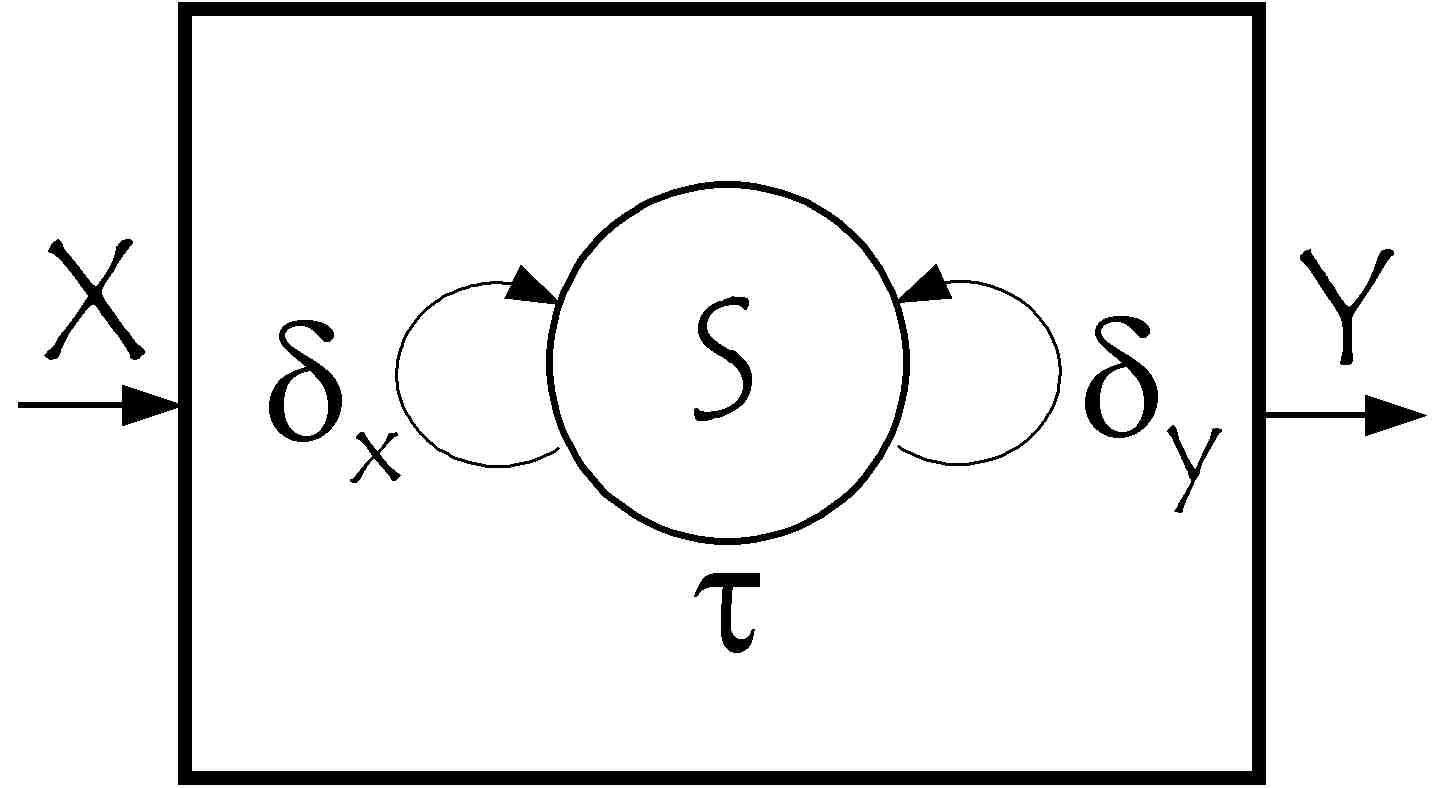
\includegraphics [width=60mm]{images/DEVSPP.jpg}}
\captionof{figure}{Dynamique DEVS}%\label{visina8}%      only if needed  
\end{minipage}

Dans ce schéma représentant le fonctionnement de DEVS, les entrées du modèle sont représentées par X, les sorties par Y, et $\delta_{x}$ la dynamique lors de la réception d'évènement, $\delta_{y}$ la dynamique interne du modèle c'est-à-dire ce qui arrive régulièrement au cours du temps $\tau$. S est l'état du système.
